\documentclass[11pt]{standalone}
\usepackage{tikz}
\usepackage{pgfplots}
\pgfplotsset{compat=1.15}
\usetikzlibrary{shapes.geometric}
\usetikzlibrary{arrows.meta,calc,decorations.pathmorphing,shapes.geometric,backgrounds,plotmarks,shapes.multipart,calc}
\begin{document} 
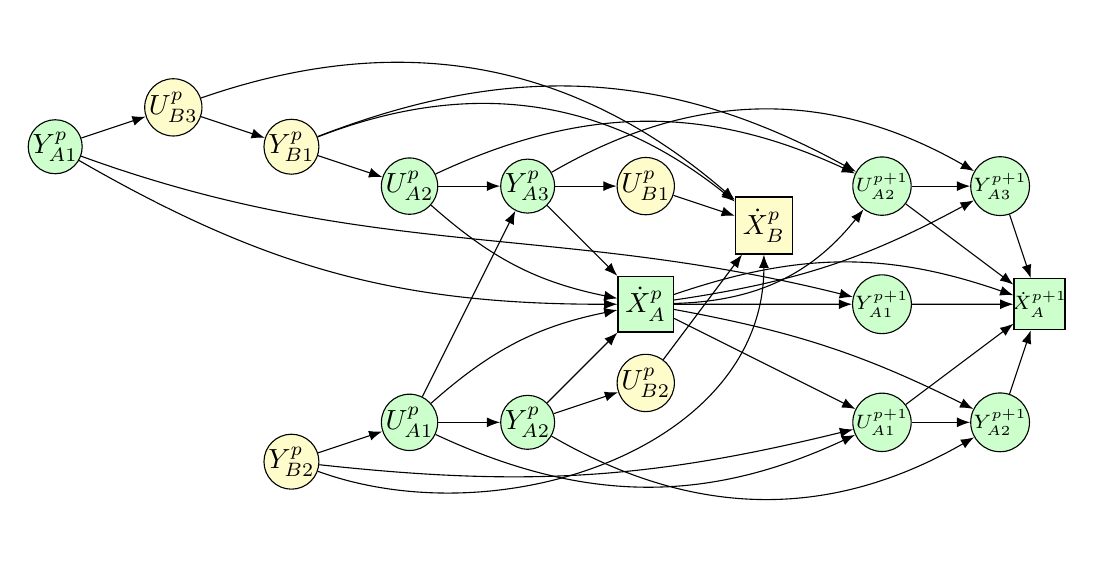
\begin{tikzpicture}

\begin{scope}[framed,local bounding box=scope1,node distance=1.5cm,operation/.style={circle,draw, inner sep = 0},square/.style={draw,regular polygon,regular polygon sides=4,inner sep=-.3}]
% Nodes
\node[operation,fill=green!20] (o5) {$Y_{A1}^p$};
\node[operation,right of = o5,yshift=.5cm,fill=yellow!20] (o4) {$U_{B3}^p$};
\node[operation,right of = o4,yshift=-.5cm,fill=yellow!20] (o8) {$Y_{B1}^p$};
\node[operation,right of = o8,yshift=-.5cm,fill=green!20] (o1) {$U_{A2}^p$};
\node[operation,right of = o1,fill=green!20] (o7) {$Y_{A3}^p$};
\node[operation,right of = o7,fill=yellow!20] (o2) {$U_{B1}^p$};
\node[square,right of = o2,yshift=-.5cm,fill=yellow!20] (o11) {$\dot{X}_{B}^p$};
\node[square,below of = o2,fill=green!20] (o10) {$\dot{X}_{A}^p$};
\node[operation,below of = o10,yshift=.5cm,fill=yellow!20] (o3) {$U_{B2}^p$};
\node[operation,left of = o3,yshift=-.5cm,fill=green!20] (o6) {$Y_{A2}^p$};
\node[operation,left of = o6,fill=green!20] (o0) {$U_{A1}^p$};
\node[operation,left of = o0,yshift=-.5cm,fill=yellow!20] (o9) {$Y_{B2}^p$};

\node[operation,right of = o11,yshift=.5cm,inner sep=0,fill=green!20] (o1_1) {\scriptsize{$U_{A2}^{p+1}$}};
\node[operation,below of = o1_1,inner sep=0,fill=green!20] (o5_1) {\scriptsize{$Y_{A1}^{p+1}$}};
\node[operation,below of = o5_1,inner sep=0,fill=green!20] (o0_1) {\scriptsize{$U_{A1}^{p+1}$}};
\node[operation,right of = o1_1,inner sep=0,fill=green!20] (o7_1) {\scriptsize{$Y_{A3}^{p+1}$}};
\node[operation,right of = o0_1,inner sep=0,fill=green!20] (o6_1) {\scriptsize{$Y_{A2}^{p+1}$}};
\node[draw,regular polygon,regular polygon sides=4,inner sep=-3.4,right of = o5_1,xshift=.5cm,fill=green!20] (o10_1) {\scriptsize{$\dot{X}_{A}^{p+1}$}};

%arcs
\path (o5) edge[-{Latex[]},bend right = 15] (o10);
\path (o5) edge[-{Latex[]}] (o4);
\path (o4) edge[-{Latex[]}] (o8);
\path (o4) edge[-{Latex[]},bend left=30] (o11);
\path (o8) edge[-{Latex[]}] (o1);
\path (o8) edge[-{Latex[]},bend left=30] (o11);
\path (o1) edge[-{Latex[]}] (o7);
\path (o1) edge[-{Latex[]},bend right=15] (o10);
\path (o7) edge[-{Latex[]}] (o2);
\path (o7) edge[-{Latex[]}] (o10);
\path (o2) edge[-{Latex[]}]  (o11);
\path (o9) edge[-{Latex[]}]  (o0);
\path (o9) edge[-{Latex[]}, out=340,in=270]  (o11);
\path (o0) edge[-{Latex[]}]  (o6);
\path (o0) edge[-{Latex[]},bend left=15]  (o10);
\path (o6) edge[-{Latex[]}]  (o3);
\path (o6) edge[-{Latex[]}]  (o10);
\path (o3) edge[-{Latex[]}]  (o11);
\path (o0) edge[-{Latex[]}]  (o7);

\path (o5_1) edge[-{Latex[]}]  (o10_1);
\path (o6_1) edge[-{Latex[]}]  (o10_1);
\path (o7_1) edge[-{Latex[]}]  (o10_1);
\path (o0_1) edge[-{Latex[]}]  (o10_1);
\path (o1_1) edge[-{Latex[]}]  (o10_1);

\path (o10) edge[-{Latex[]},bend right = 25]  (o1_1);
\path (o1) edge[-{Latex[]},bend left = 25]  (o1_1);
\path (o8) edge[-{Latex[]},bend left = 25]  (o1_1);

\path (o10) edge[-{Latex[]}]  (o5_1);
\path (o5) edge[-{Latex[]},out = 340, in = 166]  (o5_1);

\path (o10) edge[-{Latex[]}]  (o0_1);
\path (o0) edge[-{Latex[]},bend right = 25]  (o0_1);
\path (o9) edge[-{Latex[]},bend right = 10]  (o0_1);

\path (o10) edge[-{Latex[]},bend right = 10]  (o7_1);
\path (o1_1) edge[-{Latex[]}]  (o7_1);
\path (o7) edge[-{Latex[]},bend left = 30]  (o7_1);

\path (o10) edge[-{Latex[]},bend left = 8]  (o6_1);
\path (o0_1) edge[-{Latex[]}]  (o6_1);
\path (o6) edge[-{Latex[]},bend right = 30]  (o6_1);

\path (o10) edge[-{Latex[]},bend left = 19]  (o10_1);


\end{scope}

\end{tikzpicture}
\end{document}